\documentclass[a4paper,10pt]{article}

\usepackage[margin=1in]{geometry}
\usepackage{enumitem}
\usepackage[pdftex]{graphicx}
\usepackage{bbm}
\usepackage{amsfonts}
\usepackage{amsthm}
\usepackage{subfigure}

\theoremstyle{definition}
\newtheorem{defn}{Definition}
\newtheorem{obs}{Observation}

\begin{document}

\begin{enumerate}

\item Changed model slightly.  Now, model the inverse of the rate parameter, because it is more interpretable.

\item We are using generalized linear models for each of the 3 parameters.  For each parameter, the dispersion parameter is shared across patients.

\item Concerned about our prior knowledge on $\tilde{\mu}^a$, because this is our belief about the expected value of $\tilde{a}$.  

\item Key quantity of interest is $\tilde{\sigma}^a = c^a\sum_{j=1}^k \tilde{x}_j^2$

\item For a test datapoint $\tilde{x}$, prior predictive distribution of $\tilde{\mu}^a$ is unimodal if $\tilde{\sigma}^a < 1$.  So would like $\tilde{\sigma}^a$ to be less than 1 most of the time.  See Figure 1.

\item Likewise, want prior predictive distribution of $\tilde{\mu}^a$ to be unimodal.  See Figure 2.  This is always the case.  So might only worry about how the mode changes as $\tilde{\mu}^a$ changes.  See Figure 3.  Looks like if we keep $\tilde{\sigma}^c$ below 1, that would be fine.

\item  Now, interested in $\tilde{a}$ - the result of the random effect deviation from the conditional mean $\tilde{\mu}^a$.  See Figure 4.  If $\lambda^a$ is too big, the distribution of $\tilde{a}$ is no longer unimodal.  Seems like if $\lambda^a$ is greater than 10, we are fine.

\item  Likewise, interested in $\tilde{c}$ - the result of the random effect deviation from the conditional mean $\tilde{\mu}^c$.  See Figure 5.  $\lambda^c = 1$ seems fine.

\item  Finally, drew prior over curves, for different values of $\tilde{\sigma}^a=\tilde{\sigma}^b=\tilde{\sigma}^c$.  (they're not necessarily equal).  See Figure 6.


\end{enumerate}




\begin{figure}
\begin{center}
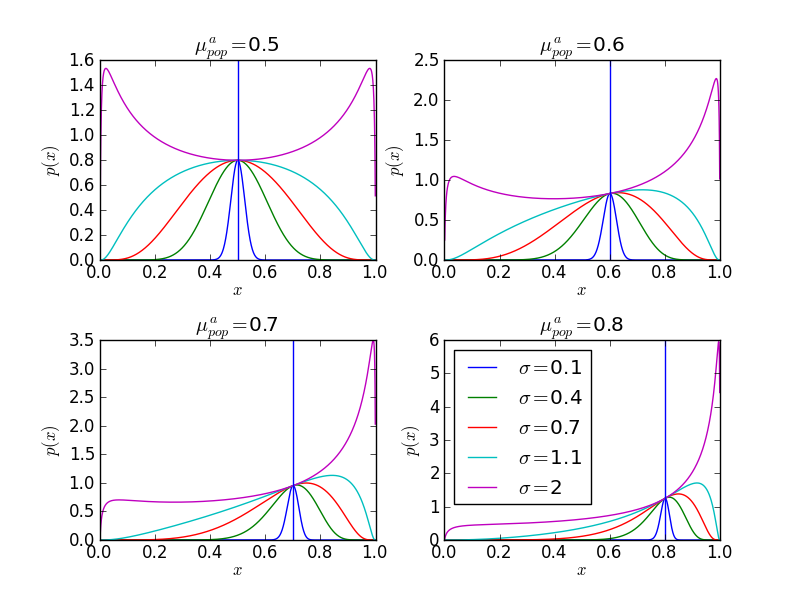
\includegraphics[width=5in, height=4in]{/Users/glareprotector/prostate_git/glare/tex_files/sections/normal_prior/files/mu_a_pdf.png}
\caption{prior predictive distribution of $\tilde{\mu}^a$ for several values of $\mu_{pop}^a$}
\end{center}
\end{figure}

\begin{figure}
\begin{center}
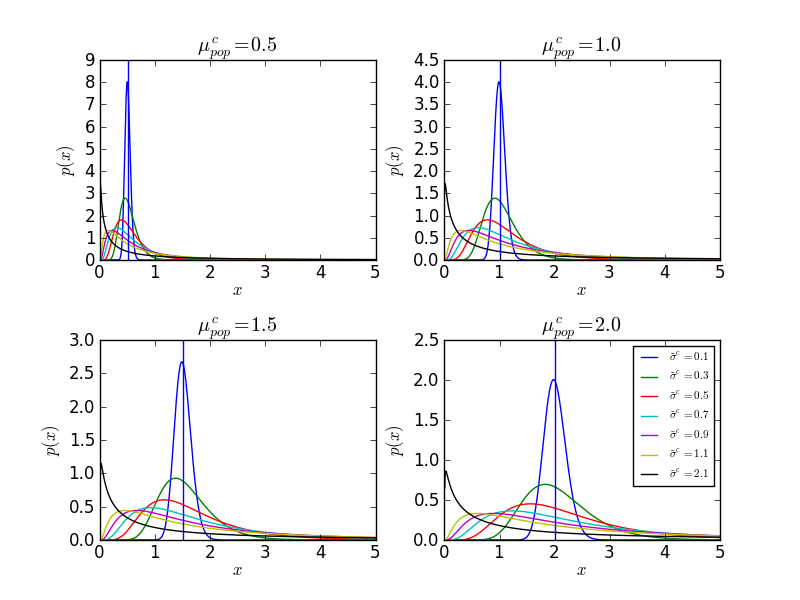
\includegraphics[width=5in, height=4in]{/Users/glareprotector/prostate_git/glare/tex_files/sections/gamma_prior/files/several_pdfs.png}
\caption{prior predictive distribution of $\tilde{\mu}^c$ for several values of $\mu_{pop}^c$}
\end{center}
\end{figure}

\begin{figure}
\begin{center}
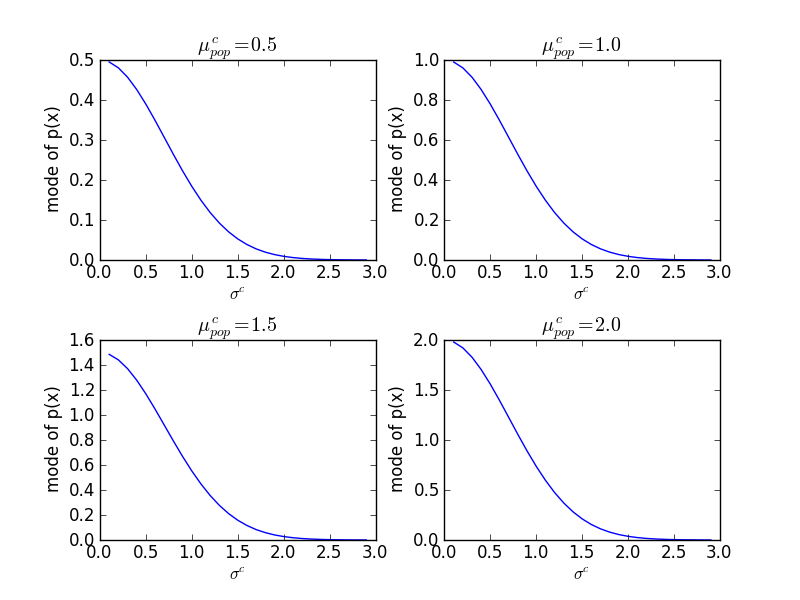
\includegraphics[width=5in, height=4in]{/Users/glareprotector/prostate_git/glare/tex_files/sections/gamma_prior/files/mode_vs_sigma.png}
\caption{Dependence of mode of $\tilde{\mu}^c$ on $\tilde{\sigma}^c $for several values of $\mu_{pop}^c$}
\end{center}
\end{figure}

\begin{figure}
\begin{center}
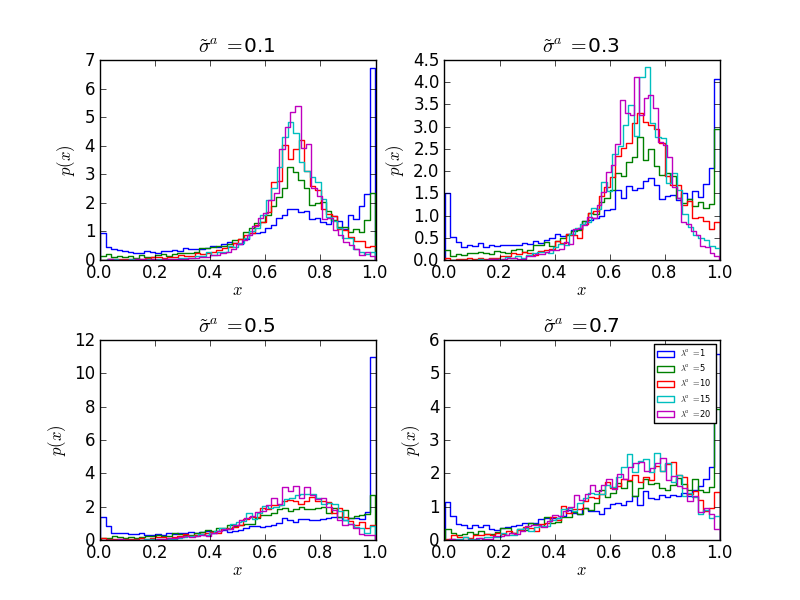
\includegraphics[width=5in, height=4in]{/Users/glareprotector/prostate_git/glare/tex_files/sections/normal_prior/files/pdf_vs_lambda_a.png}
\caption{prior predictive distribution of $\tilde{a}$ for several values of $\tilde{\sigma}^a$ and $\lambda^a$}
\end{center}
\end{figure}

\begin{figure}
\begin{center}
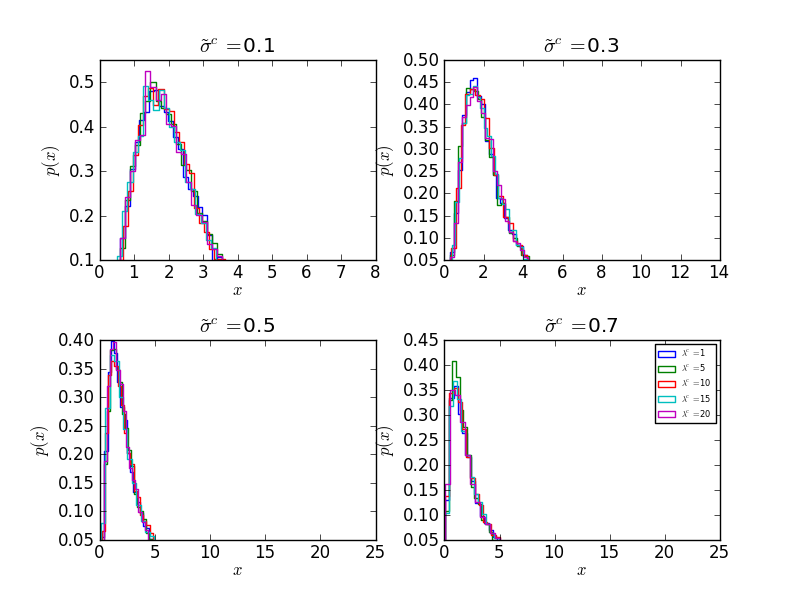
\includegraphics[width=5in, height=4in]{/Users/glareprotector/prostate_git/glare/tex_files/sections/gamma_prior/files/pdf_vs_lambda_c.png}
\caption{prior predictive distribution of $\tilde{c}$ for several values of $\tilde{\sigma}^c$ and $\lambda^c$}
\end{center}
\end{figure}

\begin{figure}
\begin{center}
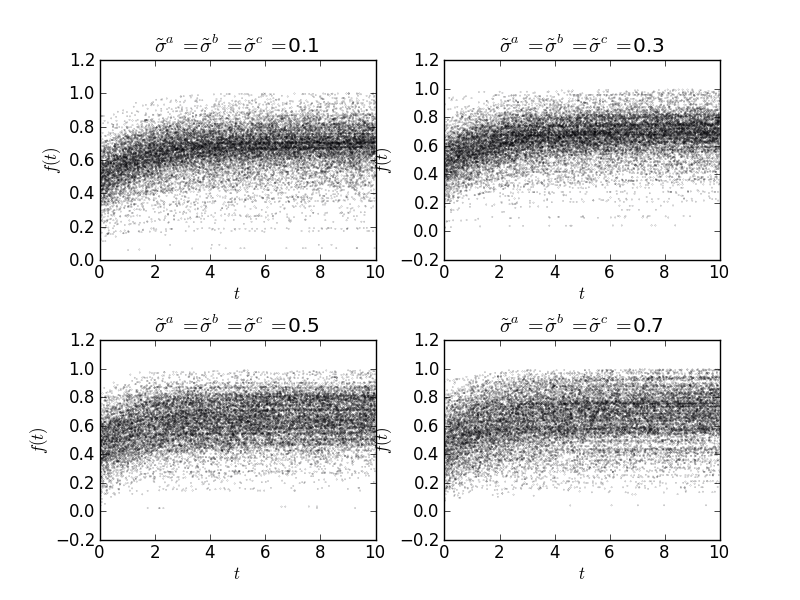
\includegraphics[width=7in, height=5in]{/Users/glareprotector/prostate_git/glare/tex_files/sections/curve_prior/files/curve_priors.png}
\caption{Curve prior for several different values of $\tilde{\sigma}^a=\tilde{\sigma}^b=\tilde{\sigma}^c$}
\end{center}
\end{figure}



\end{document}